\chapter{Technical Background}

\section{Terms and Definitions}

A Web server can be utilised to handle rather different tasks, from serving entire Web pages to representing an endpoint for raw data retrieval to merely delivering static assets like images. This section aims to give an overview of the basic requirements a modern Web server architecture needs to fulfil. Moreover, important performance factors are elaborated with regard on high-demand setups.

\subsection{Network Communication}
The eponymous task of a Web server is to serve Web-connected clients over the medium of the Internet. This involves receiving and sending messages using different implementations of network protocols. The most widely used protocol of the Web, \textit{HTTP}\footnote{Hypertext Transfer Protocol}, is a request-response protocol, which means that for every message a client sends to a server, a response is sent back \cite{http}. To minimise networking latency, it is preferable for a Web server to have a high-speed connection to the Internet, fast system I/O\footnote{\label{lab:io}Input and Output, esp. hardware} and capable routing hardware. However, these parameters are not directly related to software and are thus neglected during the further course of this thesis.

\subsection{Dynamic Content}
Originally, the Web was intended to be a network of interconnected text files, which later was augmented with images and style sheets; Web servers were basically required to understand requests and respond with static content accordingly \cite{http}. With the release of \textit{PHP}\footnote{Recursive acronym: PHP Hypertext Preprocessor, \url{http://php.net/}}, \textit{ASP}\footnote{Active Server Pages, \url{http://msdn.microsoft.com/en-us/library/aa286483.aspx}} and \textit{Java}\footnote{\url{https://www.java.com/}} -- 1995, 1996 and 1997, respectively -- dynamic webpages, i.e. views that are prepared by the server based on dynamic data like database content, became widespread \cite{webhistory}. From that point on, Web servers needed more processing capabilities for script execution and database access; however, the number of requests remained roughly the same, except for occasional form submissions \cite{webhistory}.

\subsection{Asynchronous Requests}
The advent of \textit{AJAX}\footnote{Asynchrounous JavaScript and XML (Extensible Markup Language)} and mobile applications in the late 2000's changed requirements drastically. Rather than refreshing the whole view for every piece of information sent and received, data could now be transferred in a more granular fashion. By asynchronously communicating with an API\footnote{Application Programming Interfaces} endpoint in the background, operations like deleting an item from a list could be performed invisibly and ubiquitously without reloading the page context. Especially applications that aim to provide desktop-like capabilities -- commonly called Rich Internet Applications -- make heavy use of asynchronous requests \cite[p. 4]{Sencha2011}. This inherently also changed users' expectations for websites from anticipating a certain amount of load time to implicating real-time behaviour \cite{Garrett2005}. To achieve low latency while maintaining client-server information consistency, the server's performance has to meet the combined request frequency of all clients at a given point in time.

\subsection{Request Frequency and Response Time}
Since in many cases the responsiveness of the user interface depends on the duration of the server communication roundtrip, maintaining acceptable response times is often crucial \cite[p. 1]{Nadimpalli2000}. Request frequency and response time correlate in the sense that request frequency represents the demand on a server endpoint while response time -- given equally demanding operations per request -- can be interpreted as the potential of the server to meet the demand. When the processing limit of the server is met, response times become generally inversely proportional to the request frequency, as illustrated in figure \ref{fig:response_time} \cite{response_time}. At this point, the server may chose to neglect the request (ideally by returning the status code \textit{503 Service Unavailable} \cite{http}), not respond at all or even stop serving clients altogether (i.e. ``crash'').

\begin{figure}
\centering\small
\setlength{\tabcolsep}{0mm}
  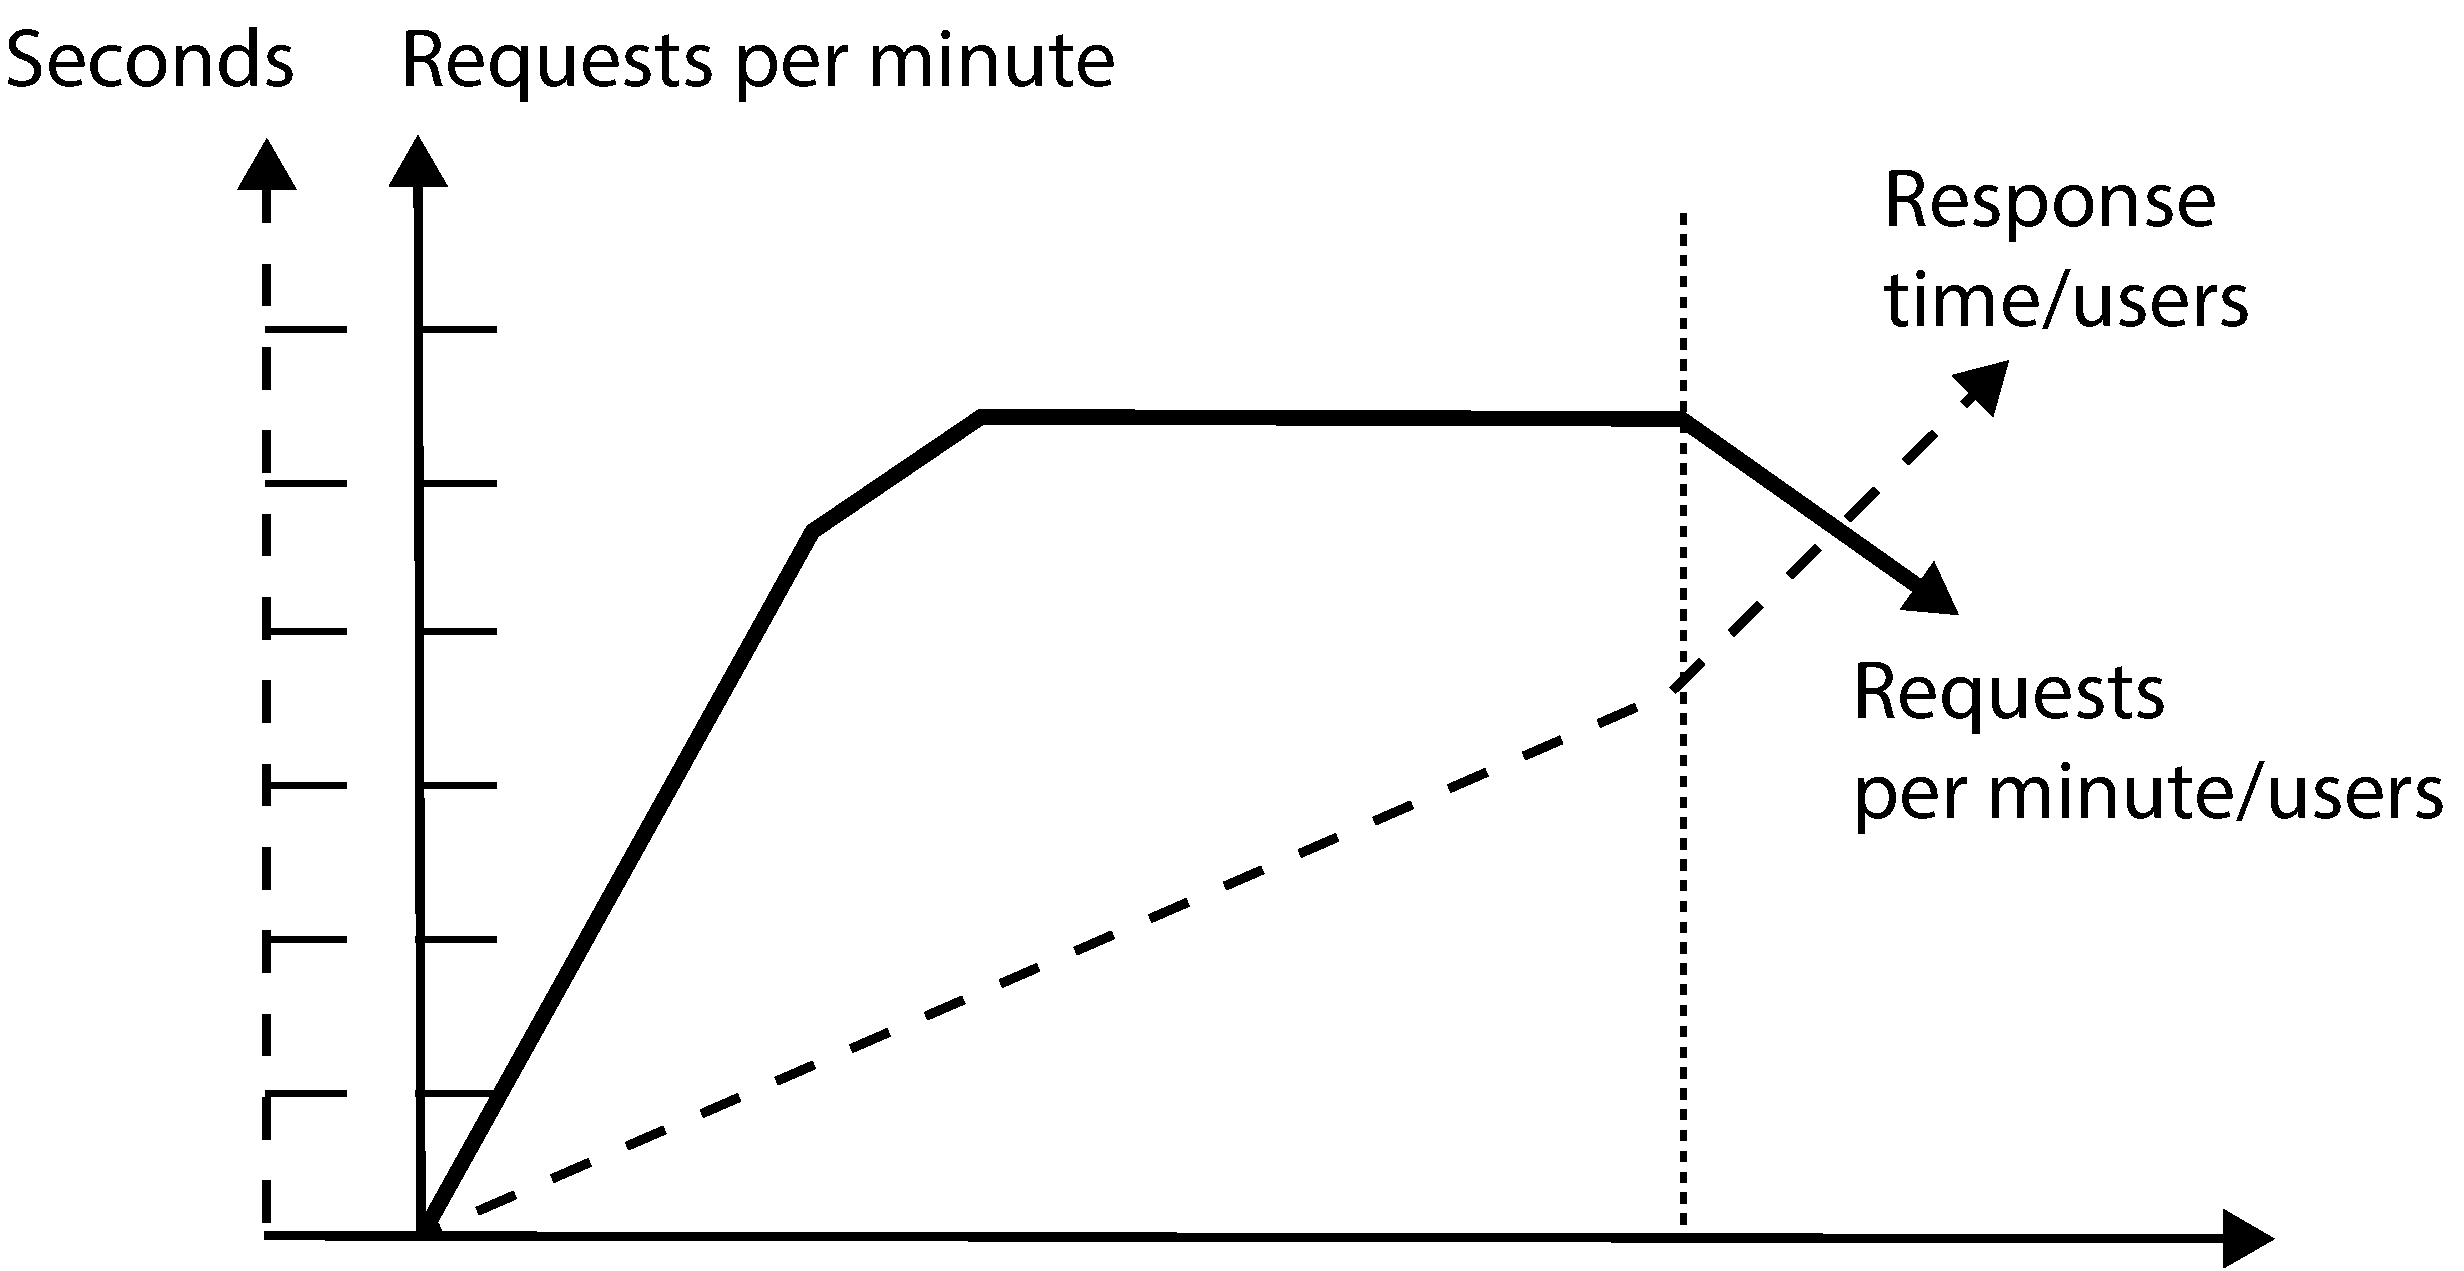
\includegraphics[width=.80\textwidth]{response_time}
\caption{
Correlation between request frequency and response time in a typical Web server setup. After the server has reached its limit of linearly serving clients (indicated by the dotted line), response times become inversely proportional to the request frequency. Image source: \cite{response_time}
}
\label{fig:response_time}
\end{figure}

\subsection{Scalability}
Demands on Web servers typically are lower during the initial phase of a business and grow with the popularity of the service. Since business growth and server load can not be exactly predicted, it is necessary to be able to adjust (i.e. \textit{scale}) the entire server architecture according to current needs in a timely manner. The \textit{Slashdot Effect} describes a sudden spike in service popularity and can, due to the open nature of the Web, lead to a tremendous increase in activity over a relatively short timespan \cite[p. 1]{Drolia2010}. 

Today's hardware is well suited to meet high demands and can be configured flexibly: If a larger number of physical server units as well as the necessary infrastructure is available, requests can be distributed and the load on a single unit decreases. If single units are outfitted with more memory and faster processors, the number of request operations per unit increases. Since acquiring and maintaining server units and other infrastructure components is expensive, well-designed software can make a significant difference in system efficiency, which in turn can greatly benefit any business \cite[p. 11]{Hughes-Croucher2012}.

Ideally, the server software should be hardware agnostic, i.e. should behave consistently independent of the hardware it runs on. For instance, if the software depends heavily on sharing application state via RAM\footnote{Random Access Memory}, scaling out on more than one machine will be unsuccessful \cite{Veal2007}. Scalability can be measured by the relationship between hardware resources and the increase of performance. If this relationship is nearly linear, the system can be considered to scale well.

\subsection{Development}
Not a part of the production system itself, but nonetheless an essential part of all Web server applications is their development. A structured, idiomatic way of writing application logic doubtlessly contributes to every software product. Modularisation of components facilitate the use of third-party software like libraries and frameworks. In return, using existing solutions can greatly reduce development time and effort, while simultaneously providing proven solutions. Web server applications particularly benefit from frameworks since they often handle standard tasks like network I/O\footnoteref{lab:io}, database access and caching \cite[Foreword]{Reelsen2011}. Integrating and maintaining these frameworks is a major part in implementing a Web server application; thus, not only the performance, but also the ease of use of selected frameworks and their language environments by the developer are treated as criteria in this thesis.


\section{Concurrency Patterns}

Since a Web application in a production setting is usually publicly accessible, serving multiple clients simultaneously is the rule, rather than the exception. Depending on the popularity of the service, the number of concurrent requests can range anywhere from dozens to several thousands, e.g. for social media sites \cite[p. 1]{Drolia2010}. A server process with a single flow of control would only be able to serve one client at once, with all requests received while the server is busy being neglected. Therefore, networking applications always have to be implemented with multiple program flows that can be executed concurrently \cite{Webopedia}. This section lists various paradigms associated with designing an application capable of maintaining multiple flows of control.

\subsection{Threads}
\label{sec:threads}
A thread is a sequence of instructions within a program. Allocating processing time to threads is handled by an operating system scheduler. To have a program execute multiple logic structures concurrently, they have to be explicitly abstracted in the form of threads. Physical concurrency occurs, when threads are executed simultaneously -- i.e. at the exactly same time -- on different processor cores; in contrast, logical concurrency describes that multiple threads are executed sequentially at roughly the same time, thus giving the impression of simultaneous execution. Physical concurrency is inherently more efficient \cite{ThreadsJava}.

\subsubsection*{Flow of Control}
A great advantage of threads in the context of Web server applications lies in the natural abstraction level regarding multiple parallel requests: Client communication is commonly treated as a set of mutually independent connections; this approach of abstraction facilitates a clear program flow structure \cite{Veal2007}. Accordingly, every request can be treated as an isolated flow of control \cite[p. 2]{Behren2003}. However, since threads are not isolated from each other and share state via a common memory address space, this only holds true as long as resources like queues or database components are accessed sequentially. Thus, close attention has to be paid by the developer to avoid race-conditions, deadlocks and access violations -- complications that generally result from improper thread coordination \cite[p. 1]{Fischer2007}. Therefore, the implementation of large-scale systems heavily relying on threads -- as an evolutionary improvement from sequential computing -- always introduces additional complexity \cite[p. 1]{Lee2006}.

\subsubsection*{Scalability}
Traditionally, Web server applications process each request on a dedicated thread throughout its whole lifespan, from accepting it to responding to it \cite[p. 162]{Henderson2006}. This behaviour can be observed for instance in implementations of the popular LAMP\footnote{Linux, Apache, MySQL, PHP} server stack configuration \cite[p. 48]{Henderson2006}. A less experienced programmer might find this ideal, since concurrency stays mostly hidden and the application logic is orientated on the flow of a single request -- smaller projects might not experience any drawbacks of this setup at all. However, it is obvious that to scale up a thread-based system the number of threads has to be increased. The number of threads engaging in simultaneous processing, i.e. physical concurrency, is limited by the number of processing cores. This means that on a computer equipped with a quad-core processor, four threads can be executed -- and thus, four requests can be served -- in parallel\footnote{Certain implementations of simultaneous multithreading allow for increasing this number at the cost of reduced performance per thread, for instance Intel's Hyper-Threading Technology (\url{http://www.intel.com/)}.}.

\subsubsection*{Problems}
Problems arise when a thread has to wait for another requirement to be fulfilled. The process of meeting a requirement that renders the executing thread unable to proceed is called a \textit{blocking} operation. Such actions include for instance reading or writing a file on mass storage, handling network traffic or file uploads, querying a database, accessing another Web service or doing intensive computations \cite[p. 196]{Henderson2006}. When a thread encounters a blocking operation, it cannot advance in the program flow until the operation completes, as illustrated in figure \ref{fig:concurrency_1}. The resulting delay can account to anywhere from a few milliseconds to several seconds, for instance when accessing a slow or irresponsive Web service. The only way to counteract the temporary occupation of threads and to continue processing incoming requests is the creation of new threads \cite[p. 36]{Hughes-Croucher2012}. However, every newly created thread counts towards certain limitations in scalability. On the one hand every thread receives a predefined share of process address space memory -- also known as \textit{stack} -- upon creation to temporarily store data \cite{Russinovich}; since memory is reserved in advance without knowing the exact requirements of the thread, a certain amount of memory overhead is likely. On the other hand, the entirety of all threads has to be orchestrated by an operating system module called \textit{scheduler}, which requires processing time relative to the number of threads \cite{Russinovich}. Moreover, a computationally expensive procedure called \textit{context switching} must also be followed upon changing the actively processed thread \cite{threads_vs_events}. 

\begin{figure}
\centering\small
\setlength{\tabcolsep}{0mm}
  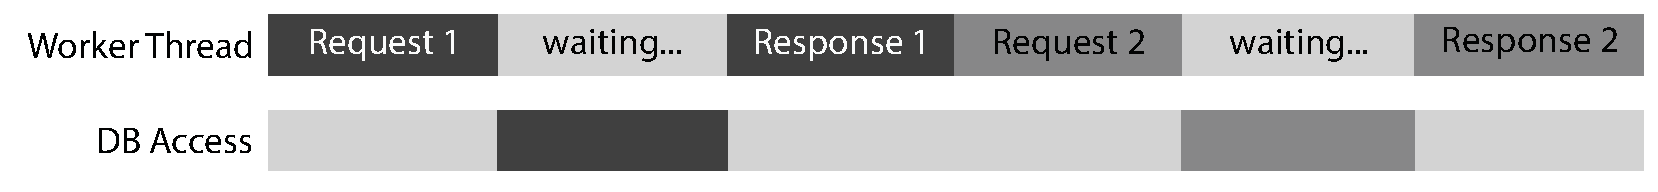
\includegraphics[width=.90\textwidth]{concurrency_1}
\caption{
A typical blocking situation in Web server scenario. When request one (shown in dark grey) arrives, a database operation is necessary. During the course of this operation, the executing thread blocks while waiting for results. The response can only be sent when data is returned and the next request (shown in medium grey) can only be served after the first one completes.
}
\label{fig:concurrency_1}
\end{figure}

Some of the problems of threads can be addressed by using a \textit{thread pool}: Instead of spawning new threads upon each request, a fixed number of threads is spawned in advanced and workload is distributed among them. However, this procedure is not without problems and introduces the delicate step of setting the thread pool size \cite{threadpools}. It can be concluded that a lower thread overhead can benefit the overall performance of a process. Furthermore, when scaling an application, the maximum number of simultaneously processed threads can at best only increase linearly in relation to the number of processing cores in a system \cite{McCool}.

\subsection{Events}
At its simplest, an event-driven application consists of two major components: On the one hand an \textit{event loop} containing an \textit{event listener} and on the other hand an \textit{event handler}. The event loop is a lightweight structure passing incoming events from a queue\footnote{A queue can theoretically be absent, but this would prevent events from being received while the event loop blocks.} to event listeners that have subscribed to a certain kind of event, e.g. an incoming network request. The targeted event listener then passes the event on to a handler function, which executes application logic and may create another event upon completion. In the case of an event-driven HTTP server, the returned event may for instance contain an HTTP response to be sent to the initial client. Larger applications typically have one event loop per process and a number of listeners and handlers \cite[p. 33]{Hughes-Croucher2012}. For an illustration of a basic event-driven application setup, see figure \ref{fig:event_loop}.

\subsubsection*{Flow of Control}
While threads present a natural abstraction for handling Web requests, recent years have seen an incline towards event-driven flow of control. Seen from a different perspective, events are at least equally idiomatic: The Web server has no control over the arriving requests, yet it has to respond by executing application logic. Instead of forcefully maintaining control over the execution context, the Web server may relinquish control and let itself be controlled by events. This strategy follows the principle of \textit{inversion of control} \cite{Hohpe2006}. 

The use of events leads to an inherently \textit{flat} application structure in the sense that there is no hierarchical ordering of event sources and destinations (see section \ref{sec:seda} for the counterpart -- staged events). There are two ways of advancing in the flow of control at the end of a particular operation: The first option is to create a new event that is received by the event loop and propagated to the next event handler. The second way is to employ a \textit{callback function}. Calling a callback function can be regarded as transferring the flow of control to an event handler without consulting the event loop \cite[p. 92]{Erb2012}. Callback functions are often used to handle results of a blocking operation -- like calling a Web service -- directly after its completion and thus maintaining control over the execution order of further actions. Implementation is typically done via either a function pointer or an \textit{annonymous function}, as demonstrated in program \ref{prog:callback1} and \ref{prog:callback2}, respectively.

\begin{program}
  \caption{Calling a callback function via a function pointer in JavaScript.}
  \label{prog:callback1}
  \begin{JavaCode}
function callbackFunction (data) {
    console.log(data);
}
  
WebService.get("http://example.com/").then(callbackFunction);
  \end{JavaCode}
\end{program}

\begin{program}
  \caption{Calling a callback function via an annonymous function in JavaScript.}
  \label{prog:callback2}
  \begin{JavaCode}
WebService.get("http://example.com/").then(function(data) {
    console.log(data);
});
  \end{JavaCode}
\end{program}

Instead of keeping the entirety of method calls leading to a certain behaviour in a section of reserved memory called the \textit{stack}, event-driven programming makes use of \textit{callback functions}.   

\subsubsection*{Relation to Threads}

Event-driven programming does not preclude the existence of threads; neither is it the opposite or an evolutionary step. All major operating systems use threads as a means of managing process execution, thus even a purely event-driven program needs at least one thread. However, this is not a favourable scenario, especially for a Web server: If the event loop and the handler would run on the same thread, the event loop would block if the handler blocks and thus would not be able to accept further events. Therefore the event loop (and with it the application I/O\footnoteref{lab:io}) commonly runs on a dedicated thread with the handlers run on other threads or -- in more sophisticated implementations -- in a thread pool (see section \ref{sec:threads}). 

\begin{figure}
\centering\small
\setlength{\tabcolsep}{0mm}
  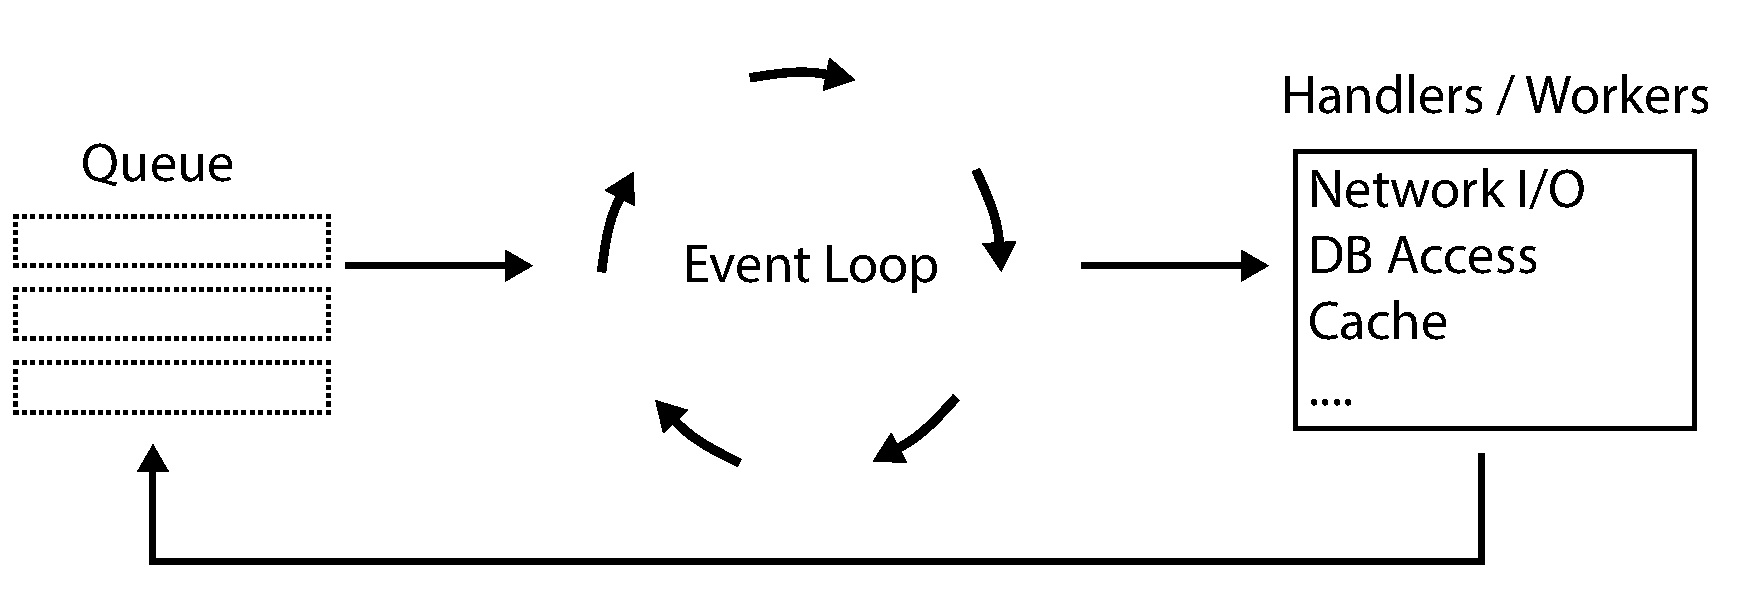
\includegraphics[width=.80\textwidth]{event_loop}
\caption{
Basic flow of control in an event-driven application. Operations that would normally block the event loop are executed separately and create further events upon completion.
}
\label{fig:event_loop}
\end{figure}

\subsection{SEDA}
\label{sec:seda}

In this thesis, the term \textit{event-driven} always describes intra-system event architecture, also known as \textit{staged event-driven architecture} (\textit{SEDA}) \cite{event-architecture}.

When incoming demand exceeds system processing capacity, it can simply queue up requests in its internal buffer queues.

\subsection{Actors}

\subsection{Reactive Architecture}

























